%%%%%%%%%%%%%%%%%%%%%%%%%%%%%%%%%%%%%%%%%%%%%%%%%%%%%%%%%%%%%%%
%
% Welcome to Overleaf --- just edit your LaTeX on the left,
% and we'll compile it for you on the right. If you open the
% 'Share' menu, you can invite other users to edit at the same
% time. See www.overleaf.com/learn for more info. Enjoy!
%
%%%%%%%%%%%%%%%%%%%%%%%%%%%%%%%%%%%%%%%%%%%%%%%%%%%%%%%%%%%%%%%
\documentclass{beamer}

\usetheme{Madrid}
\usecolortheme{lily}
\addtobeamertemplate{footnote}{}{\vspace{2ex}}

\usepackage{amsmath}
\usepackage{amssymb}
\usepackage{color}
\usepackage{listings}
\usepackage{clrscode3e}
\usepackage{multicol}

\definecolor{codegreen}{HTML}{237e02}
\definecolor{codegray}{rgb}{0.5,0.5,0.5}
\definecolor{codepurple}{HTML}{8F4673}
\definecolor{codebrown}{HTML}{ce9178}
\definecolor{codecyan}{HTML}{098658}
\lstdefinestyle{pythonstyle}{
    commentstyle=\color{codegreen},
    keywordstyle=\color{codepurple},
    numberstyle=\tiny\color{codegray},
    stringstyle=\color{codebrown},
    basicstyle=\ttfamily\small,
    breakatwhitespace=false,         
    breaklines=true,                 
    captionpos=b,                    
    keepspaces=true,                 
    numbersep=5pt,                  
    showspaces=false,                
    showstringspaces=false,
    showtabs=false,
    tabsize=2
}
\def\And{\text{ AND }}
\def\Or{\text{ OR }}
\def\Xor{\text{ XOR }}
\def\Implies{\text{ IMPLIES }}
\def\Iff{\text{ IFF }}
\def\Not{\text{NOT}}
\def\R{\mathbb{R}}
\def\N{\mathbb{N}}
\lstset{style=pythonstyle}

\setlength{\parskip}{1em}

%Information to be included in the title page:
\title{Format for Efficient Storage of Homology Relations}
\subtitle{Week 1-2 Report: Comparing Existing Implementations and Approaches}
\author{Kevin Gao}
\institute{University of Toronto}

\begin{document}

\frame{\titlepage}

\AtBeginSection[]
{
    \begin{frame}
    \frametitle{Outlines}
    \tableofcontents[currentsection]
    \end{frame}
}

\section{Existing Formats for Homology Data}

\begin{frame}{Overview}
    Various file formats exist for storing homology data. In general, these formats fall into the following categories:

    \begin{itemize}
        \item Direct storage of each pair (usually in a relational database)
        \item Semi-structured data (e.g. JSON, XML, and their variations)
        \item Newick format (and others based on Newick such as New Hampshire X format and Extended Newick)
    \end{itemize}

    Some other less common data representations include
    \begin{itemize}
        \item Edge list, adjacency matrix, etc.
        \item Human-readable flatfile
    \end{itemize}
\end{frame}

\begin{frame}{Relational Database Approach}
    As discussed in our last meeting and my project proposal, the current way homology data is stored in a relational database as pairs.

    Each pair $(x,y,\text{type})$ denotes that $x$ is homologous to $y$ of type `type': 
    
    `ortholog\_one2one',`ortholog\_one2many',\\`ortholog\_many2many',`within\_species\_paralog', `gene\_split', etc.
    
    Each node is also associated with additional information such as the Jaccard coefficient.
\end{frame}

\begin{frame}{XML}
    Two of the most commonly used semi-structured data formats are JSON and XML. In particular, XML is often used for phylogenetic and other bioinformatics data due to their hierarchical structures, allowing them to be easily interpreted as a tree.

    PhyloXML is one XML schema that encodes phylogenetic trees. It is a suitable candidate for our project on alternative and efficient representations for homology data.
\end{frame}

\begin{frame}{Newick}
    Newick format uses parenthesization to represent hierarchical data. Given a tree, a string of balanced parentheses can be generated using a DFS. Newick is compact and records only the minimal amount of information. With appropriate encoding of node labels, Newick format can achieve a file size close to the information theoretical lower bound.

    \begin{figure}[htbp]
        \centering
        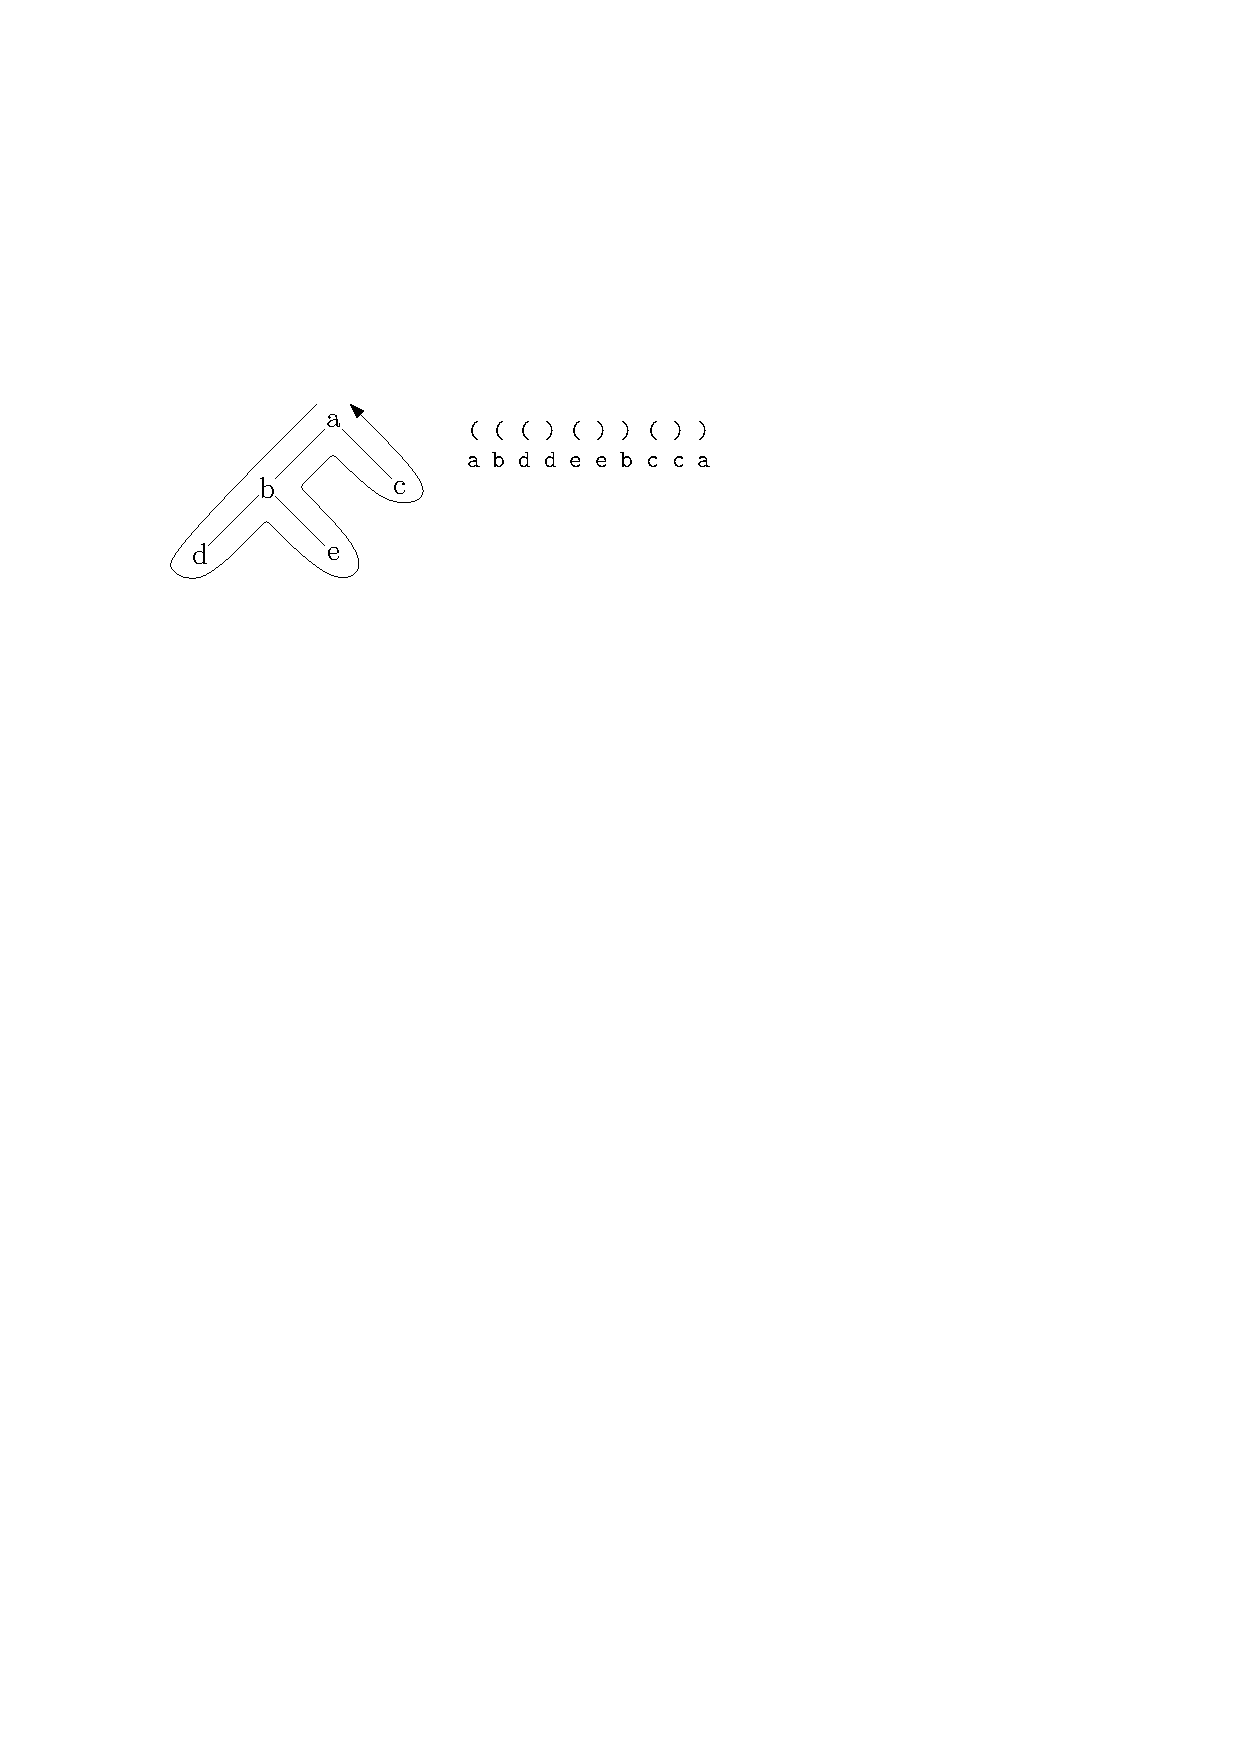
\includegraphics[width=0.5\linewidth]{res/balanced-paren.pdf}
        \caption{Balanced parenthesis generated from the DFS of the tree on the left.}
        \label{fig:parentheses}
    \end{figure}
\end{frame}

\begin{frame}
    \begin{figure}[htbp]
        \centering
        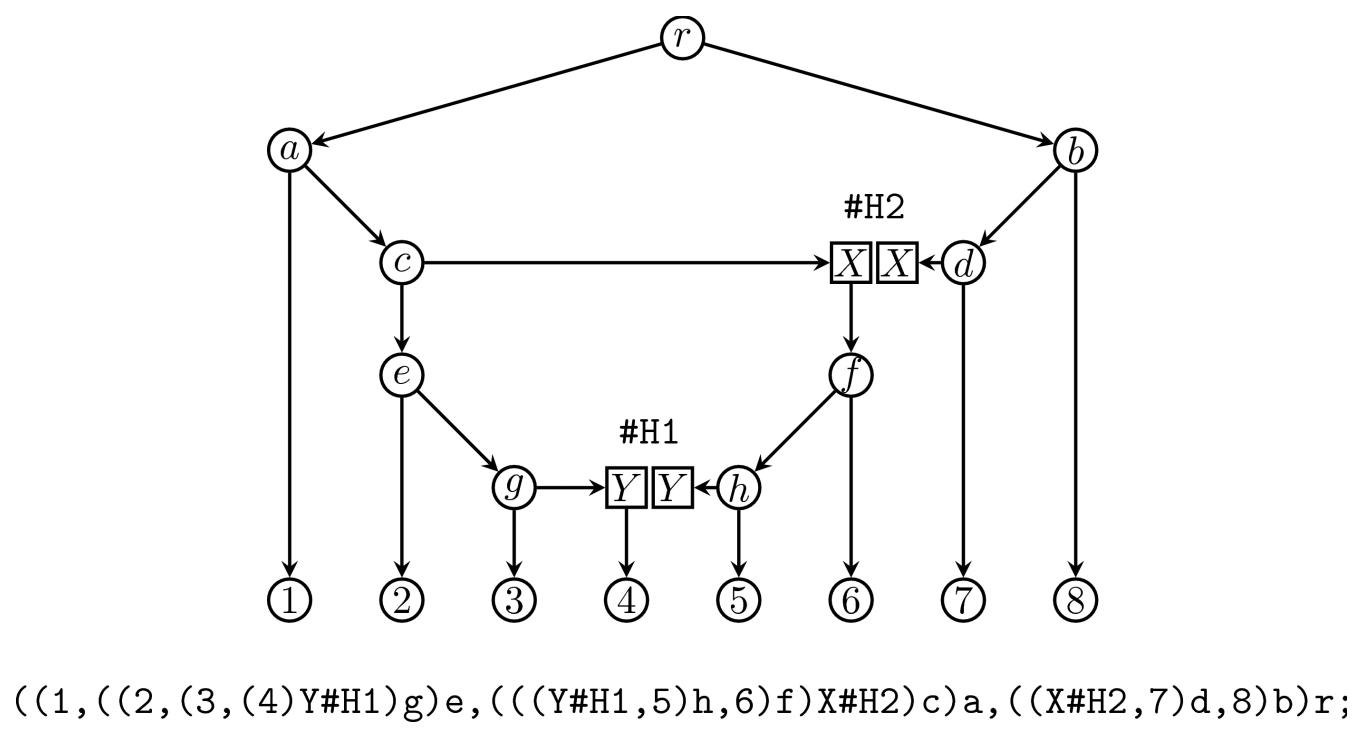
\includegraphics[width=0.7\linewidth]{res/newick.png}
        \caption{A phylogenetic tree and its corresponding Newick format.}
        \label{fig:newick}
    \end{figure}
\end{frame}

\section{PhyloXML}

\begin{frame}{XML and Parsing}
    The bottleneck when using XML for large dataset is parsing XML file to the corresponding data structures so that we can run queries. Before the data can be accessed and queried, the XML file needs to go through lexical analysis and syntactic analysis.

    At the end of parsing, a representation of the original XML file is generated, usually using one of the three models:
    \begin{itemize}
        \item DOM (document data model): creates a tree that is stored directly in the memory for access
        \item VTD (virtual token descriptor): stores the original file and arrays of 64-bit integers of token positions and parent-child-sibling relationship among tokens
        \item SAX (simple API for XML) and StAX (streaming API for XML): do not directly store long-lived data structures in memory and instead use streaming and online algorithms for query
    \end{itemize}
\end{frame}

\begin{frame}
    DOM and VTD both store long-lived data structures in the memory. This provides easier and more direct query of data, along with the ability to index the data. But these approahces can be impractical for extremely large datasets.

    SAX and StAX associate objects with ``events'': start element event denoting the beginning of a node, end element events denoting the end of a node. Because of this, access is often limited to sequential access. More complex queries like LCA and those often used in bioinformatics require online algorithms.
\end{frame}

\begin{frame}
    Figures on the next two pages are from 
    
    {T. C. Lam, J. J. Ding and J. Liu, "XML Document Parsing: Operational and Performance Characteristics," in Computer, vol. 41, no. 9, pp. 30-37, Sept. 2008, doi: 10.1109/MC.2008.403.}
\end{frame}

\begin{frame}
    \begin{figure}[htbp]
        \centering
        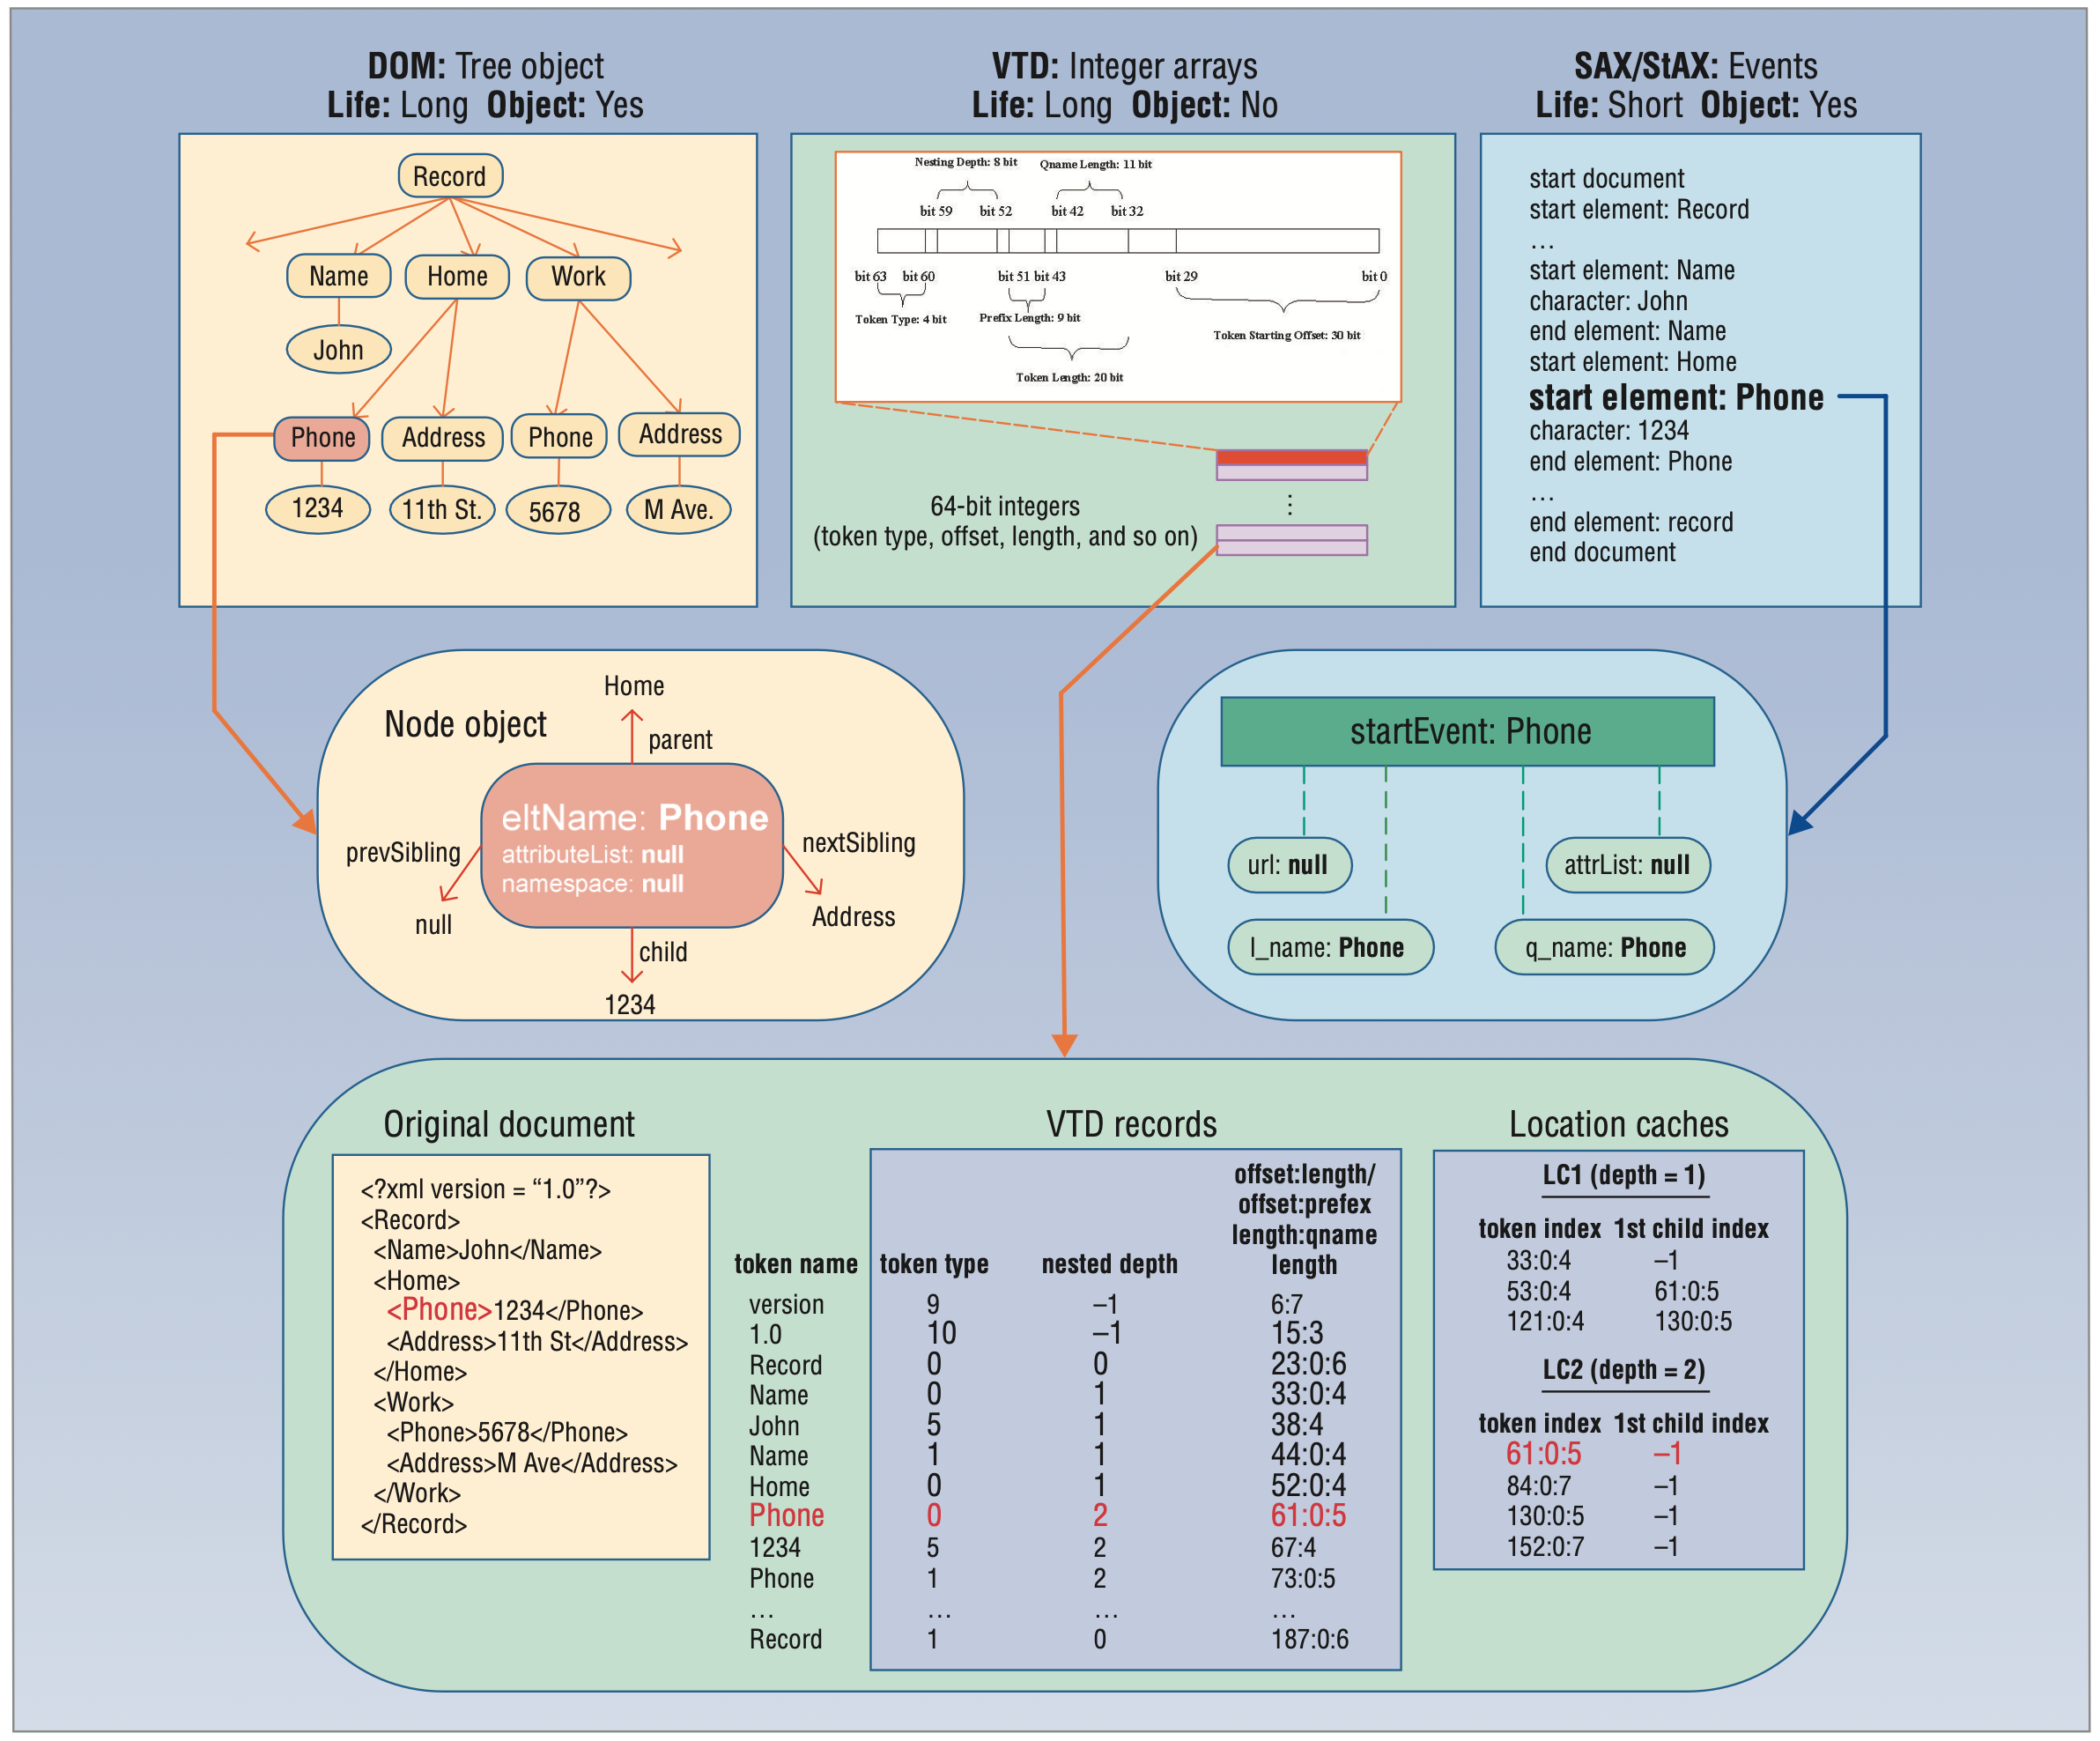
\includegraphics[width=0.7\linewidth]{res/xml-parsing-models.png}
        \caption{Overview of the three main XML parsing models.}
        \label{fig:xml-parsing-models}
    \end{figure}
\end{frame}

\begin{frame}
    \begin{figure}[htbp]
        \centering
        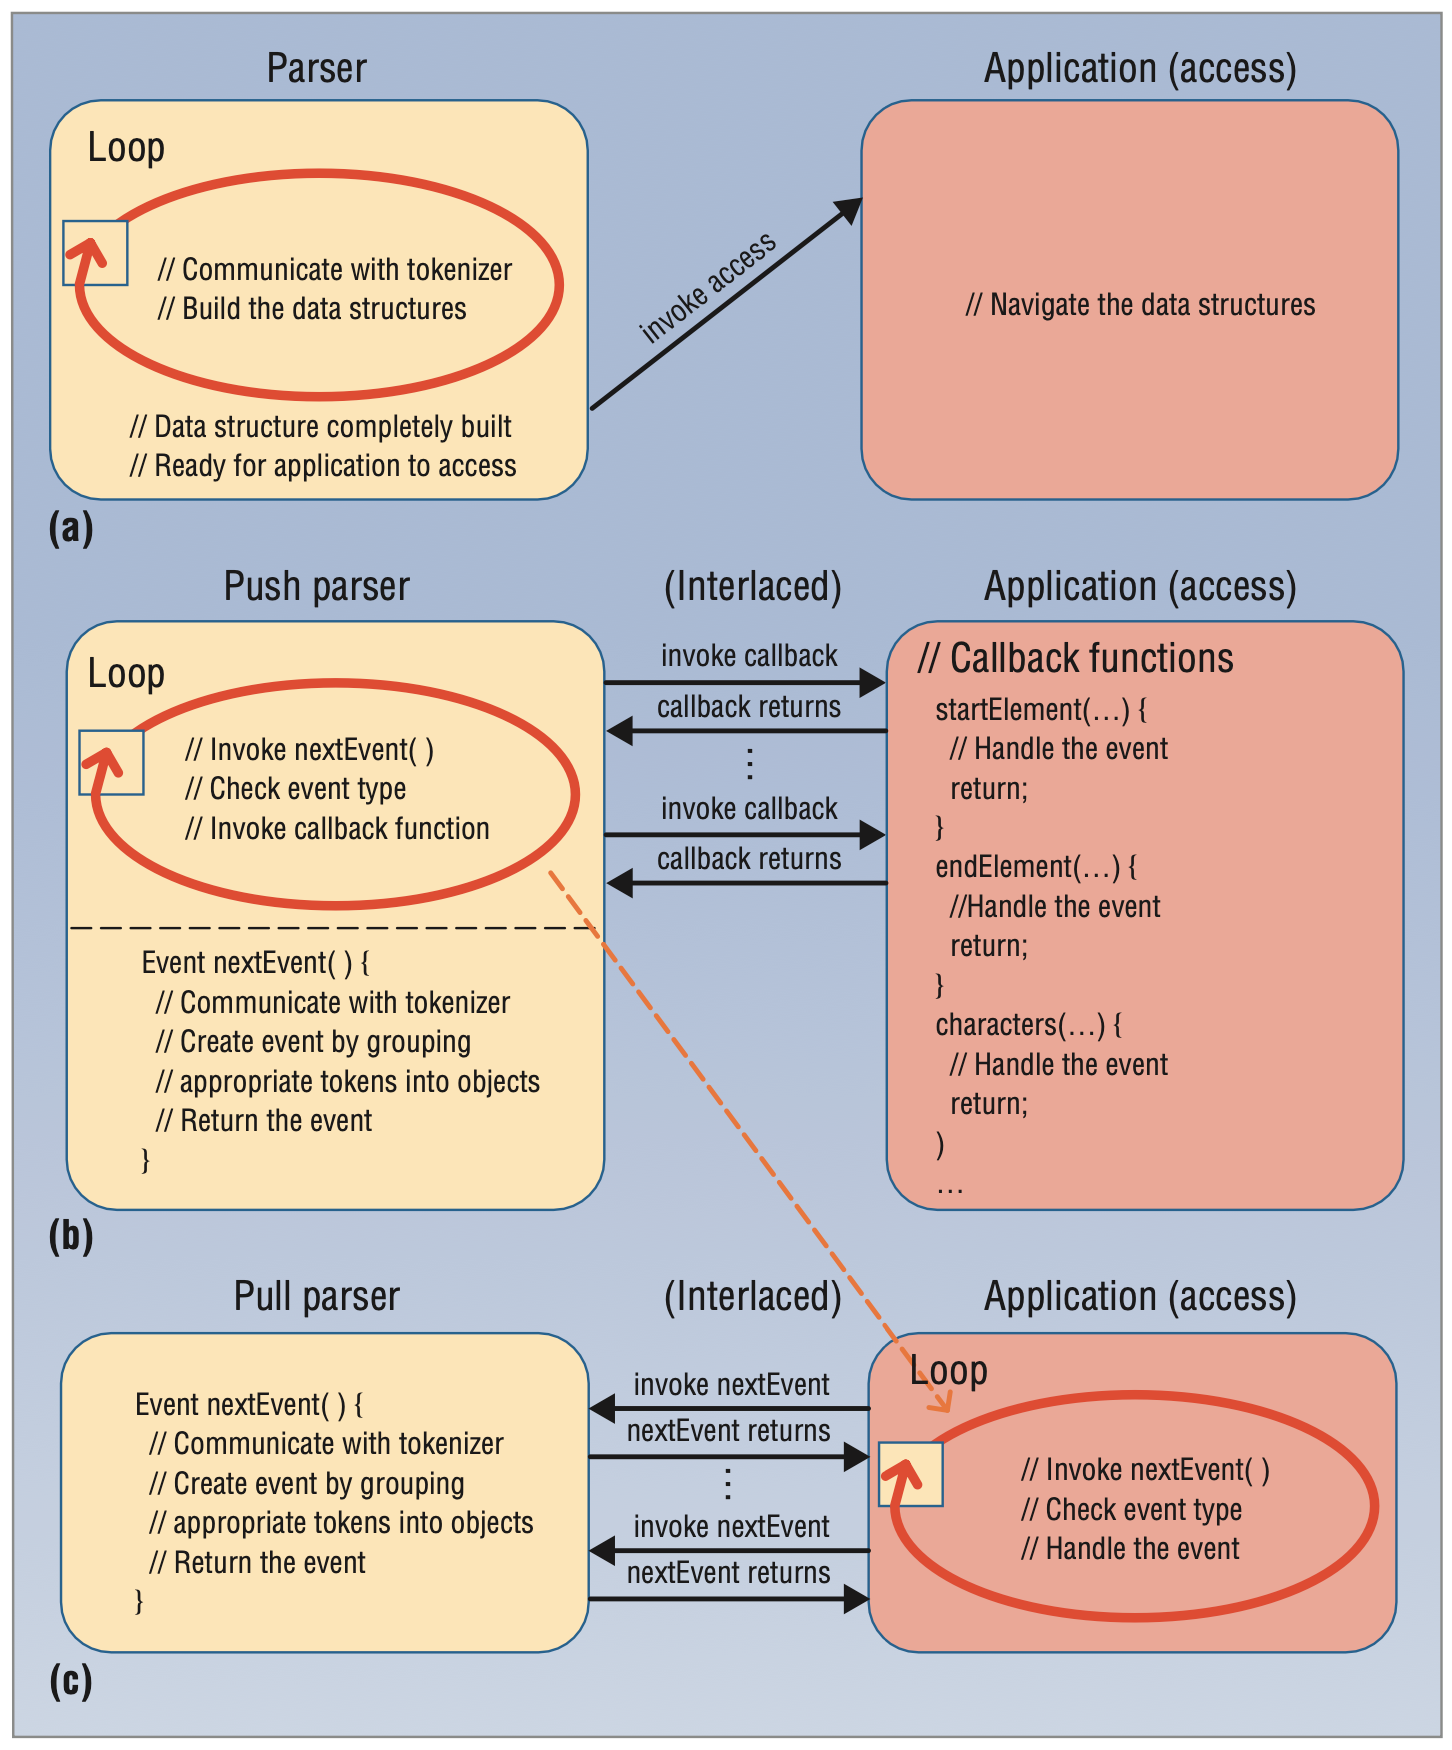
\includegraphics[width=0.5\linewidth]{res/xml-parsing-interaction.png}
        \caption{Interaction between the parser and application (APIs for accessing and querying). (a) DOM and VTD; (b) SAX; (c) StAX.}
        \label{fig:xml-parsing-interaction}
    \end{figure}
\end{frame}

\begin{frame}{Indexing XML}
    Ideally, without memory limitation, \textbf{VTD} would be the best candidate for our implementation since it keeps track of a \textbf{location cache (LC)} for parent-child-sibling relationship among the tokens.

    The result of parsing using the VTD model can also be used as an index for faster query.
\end{frame}

\begin{frame}{Indexing XML (or trees, in general)}
    An alternative and interesting way to index a tree for fast ancestor queries is to label the nodes using some specific \textbf{labeling schemes}.
    
    Each node, apart from the existing attributes such as name, identifier, etc., will have a label such that given two labels, one can quickly determine the structural relationship of the nodes assocaited with the two labels within a tree.
    
    For better performance and memory efficiency, we can instead index a tree with only the labels and use a labeling scheme that gives us labels with shorter lengths.
\end{frame}

\begin{frame}
    In their paper \textit{A Comparison of Labeling Schemes for Ancestor Queries}, Kaplan, Milo, and Shabo introduced some labeling schemes that are used in actual database systems and also proposed new methods for creating labels for indexing. Most labeling schemes reduces the problem of an ancestor query in the tree to string comparisons (such as interval containment, prefix testing, etc.)

    \begin{itemize}
        \item Recursive labeling scheme (Santoro and Khatib): $\log n + O(\sqrt{\log n})$
        \item Compressed prefix scheme (Kaplan, Milo, and Shabo): $O(\log n)$
        \item Hybrid 2-level scheme (Kaplan, Milo, and Shabo): $\frac{3}{2} \log n + O(\log \log n)$ 
    \end{itemize}

    This paper by Kaplan et al. provides us with insights to some possible ways for implementing the parser and index to reduce the memory usage and make queries more efficient later on in the project.
\end{frame}

\section{Newick Format}

\begin{frame}{Newick}
    Due to its compact size, parsing a Newick format file into the memory is likely going to be faster than XML. But it has several drawbacks:
    \begin{itemize}
        \item Newick format on its own does not encode structural information about the tree directly, making complex queries harder and more costly
        \item Newick format only supports rooted tree, which may or may not be the case for homology data
    \end{itemize}
    The first issue can be problematic since the majority of the queries regarding homology data is determining the ancestry/structural relationship of two nodes in the tree. This means if we use Newick for our format, we would need to use some of the \textbf{encoding schemes} mentioned earlier to \textbf{index} the tree.
\end{frame}

\begin{frame}{Newick Format in Practice}
    \textbf{TreeBASE} was a repository of phylogenetic information. Detailed information about the nodes is stored in a relational database but structural data about the phylogenetic tree is kept in a file encoded in Newick format. A TreeBASE query requires first a query in the relational database, followed by a query outside the database on the tree encoded in Newick format.

    Given the drawbacks of Newick format, a well-designed index is likely required. But the overall architecture of the database is similar to what we are aiming for.
\end{frame}

\begin{frame}
    Nakhleh et al. described in their paper\footnote{L. Nakhleh, D. Miranker and F. Barbancon, "Requirements of phylogenetic databases," Third IEEE Symposium on Bioinformatics and Bioengineering, 2003. Proceedings., 2003, pp. 141-148, doi: 10.1109/BIBE.2003.1188940.} an alternative to Newick format -- to store the edges of the tree directly in a relational database.

    The authors claim that LCA queries can be done quite efficiently in practice. The benchmark results in the paper can be used as a reference when evaluating the performance of our format.
\end{frame}

\section{Queries}

\begin{frame}{Common Types of Queries}
    The author of the paper mentioned in the previous slide also outlined some of the common type of queries on a database of homology data:
    \begin{itemize}
        \item Common ancestor (CA) and lowest common ancestor (LCA) of two nodes
        \item Path length between two nodes
        \item Distance between two leaves
        \item Minimum spanning clades of a given set of taxa
    \end{itemize}
    It is important to keep in mind these common queries when evaluating the performance and efficiency of our data format.
\end{frame}

\section{References}

\begin{frame}
    \scriptsize

    T. C. Lam, J. J. Ding and J. Liu, "XML Document Parsing: Operational and Performance Characteristics," in Computer, vol. 41, no. 9, pp. 30-37, Sept. 2008, doi: 10.1109/MC.2008.403.

    Haim Kaplan, Tova Milo, and Ronen Shabo. 2002. A comparison of labeling schemes for ancestor queries. In Proceedings of the thirteenth annual ACM-SIAM symposium on Discrete algorithms (SODA '02). Society for Industrial and Applied Mathematics, USA, 954-963.

    L. Nakhleh, D. Miranker and F. Barbancon, "Requirements of phylogenetic databases," Third IEEE Symposium on Bioinformatics and Bioengineering, 2003. Proceedings., 2003, pp. 141-148, doi: 10.1109/BIBE.2003.1188940.

    Cardona, G., Rossello, F. and Valiente, G. Extended Newick: it is time for a standard representation of phylogenetic networks. BMC Bioinformatics 9, 532 (2008). https://doi.org/10.1186/1471-2105-9-532

    Kmettlca, E.A. O(log n) persistent online lowest common ancestor search without preprocessing. https://github.com/ekmett/lca/
    
    Wansong Zhang, Daxin Liu and Jian Li, "An encoding scheme for indexing XML data," IEEE International Conference on e-Technology, e-Commerce and e-Service, 2004. EEE '04. 2004, 2004, pp. 525-528, doi: 10.1109/EEE.2004.1287357.
\end{frame}

\end{document}